\Chapter{Technikai kivitelezés}
Ebben a fejezetben bemutatom az elkészült programot a számomra legérdekesebb programrészletekkel. Nem térek ki minden funkcióra és programkódra, csak a lényegesebb egységekre. Részletezem a front end kivitelezését, amelybe tartozik a Vue JS, HTML és CSS kódok. Ezután a back end számításokat mutatom be, amelyet Node JS környezetben valósítottam meg.

\section{A projekt felépítése}
Mielőtt belekezdek a megoldásaim, függvények, programkódok magyarázásába, először bemutatom a projekt felépítését, hogy egyszerűbben érthető legyen. Először a webalkalmazás felépítését mutatom be. 

A webalkalmazás frontend részét a már említett Vue JS-ben valósítottam meg. Ebben vannak a komponensek és a vue-router, amely az oldalak közti mozgást végzi el. A front end és a back end közötti kommunikációt az API végzi. A JSON adatbázis lokálisan helyezkedik el és csak a back end kommunikál vele, illetve használja a számításokhoz.

\begin{figure}[h]
\centering
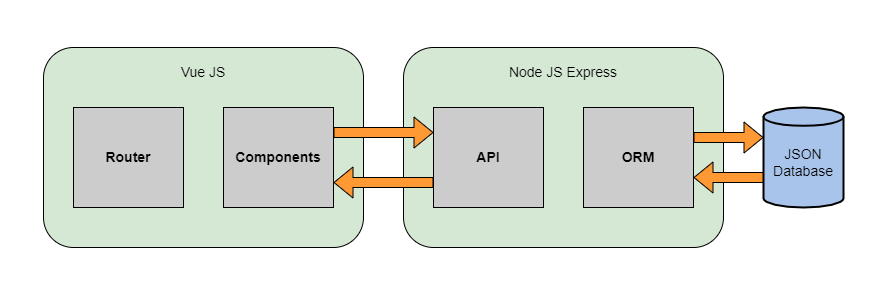
\includegraphics[scale=0.8]{images/web-arch.png}
\caption{A webalkalmazás architektúrális ábrája}
\label{fig:web-arch}
\end{figure}

A 3.2-es ábrán látható az elkészült projekt struktúrája file rendszer szinten. Az ábra bal oldalán a front end felépítése látható. A components mappában vannak a komponensek, amelyeket többször fel lehet használni az oldalakon. 

A router mappában lévő index.js file-ban vannak definiálva a router-ek. Itt meg kell adni az elérési útvonalat, az oldal nevét, amelyre irányítani szeretnénk a felhasználót, illetve importálni az adott vue file-t. Ezeket az oldalakat a views mappában találjuk, itt az autentikációt végző oldalak, a home fül és a SimulateGame helyezkedik el, amelyben maga a póker alkalmazás valósul meg.

Ezeken kívül a main.js-ben importálni kell minden olyan kiegészítőt, melyet használok az alkalmazásban, valamint a Firebase config része is itt van definiálva. Fontosak még az css file-ok, ezeket importálom be az egyes oldalakon, hogy a megfelelő megjelenést kölcsönözzem nekik. Ezeken kívül a package.json és package-lock.json file-okban meg vannak adva a felhasznált technológiák verziója, hogy ne legyen köztük ütközés.

Az ábra jobb oldalán látható az alkalmazás back end része. Itt az erchitektúra jóval egyszerűbb. Két json adathalmazt hoztam létre, az egyik a kártyák erősségét tárolja, a másik a preflop esélyeket, mind a kettőben egy-egy objektum helyezkedik el. Itt is megtalálható a package.json és a package-lock.json, ezek ugyanazt a szerepet töltik be, mint a front end-nél. Az index.js is hasonló mint a front end-en, itt is be kell importálni minden felhasznált technológiát, valamint megadni, hogy milyen porton fusson a back end. Erre azért van szükség, hogy a localhost-on futtatott kliens és szerver ne kavarodjon össze.

A findStrongest.js-ben azok a kódok vannak, melyek a felhasználó esélyeit vizsgálják, a findEnemyStrongest.js-ben pedig azok, amik az ellenfél esélyeit. A helperFunctions.js arra szolgál, hogy a több helyen meghívott függvényeket eltárolja, így azokat nem kell többször megírni. Végül a root.js-ben két post response helyezkedik el, így történik az adatátvitel a kliens részére.

\begin{figure}[h]
\centering
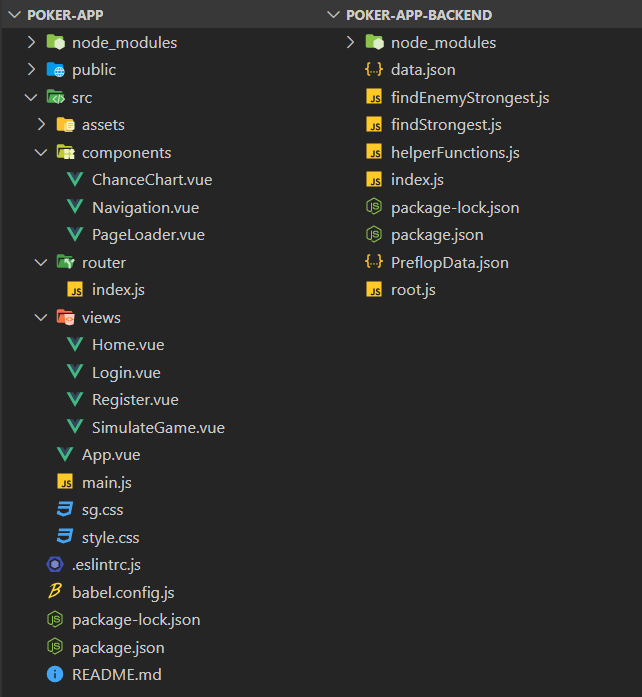
\includegraphics[scale=0.8]{images/frontend-backend-arch.png}
\caption{A projekt struktúrája file rendszer szinten}
\label{fig:frontend-backend-arch}
\end{figure}

Az osztály diagrammon bemutatom, hogy nagy vonalakban milyen adatokkal, fügvényekkel és a hozzájuk kapcsolódó paraméterlistákkal dolgoztam. Ez a 3.3-as ábrán látható. A kék elem a klienst szemlélteti, a sárgák pedig a szervert hivatottak bemutatni.

Az adatok mindenhol tartalmazzák a sevenCards és az everyCards adatokat, kivéve a helperFunctions-nál, hiszen onnan csak meghívom a függvényeket. A front end oldalon továbbá jelen van a myCards is, erre az esélyek ábrázolása miatt van szükség. Itt jelenítem meg a diagrammokat a chartCalc függvénnyel. A chooseCard függvény veszi ki a lapokat a pakliból, amit majd továbbadok a szervernek, valamint a lapok megjelenítésében is szerepet játszik. A két backend függvény pedig két post request-et tartalmaz.

A sárga részeken találhatóak azok az adatok és függvények, amik az esélyek számolásáért felelősek. A teljesség igénye nélkül, itt számolom a lehetséges érkező lapokat, ezekre az értékeket, sorba rendezem a lapokat, leszűkítem csak a nevekre, és egyéb lent látható eseményeket.

\begin{figure}[h]
\centering
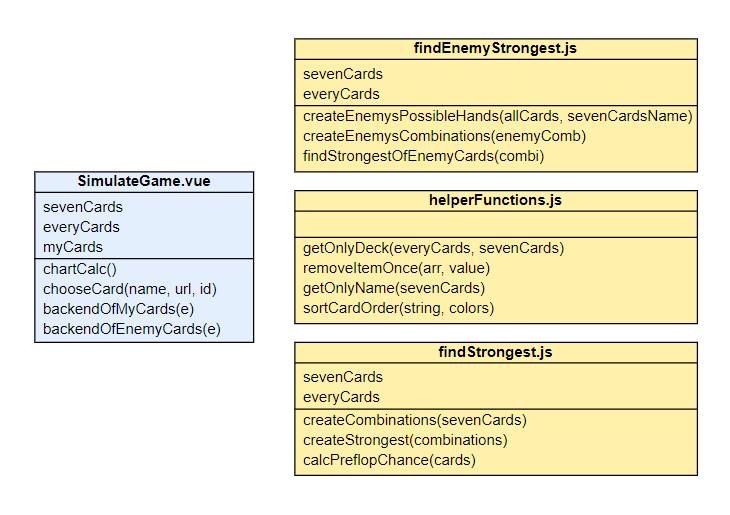
\includegraphics[scale=0.9]{images/class-model.png}
\caption{Az alkalmazás osztály diagrammja}
\label{fig:class-model}
\end{figure}

\section{Front end kivitelezése}
Egy webalkalmazás front end része az, amit a felhasználó érzékel az oldalról. Itt részletesen bemutatom a főbb egységeket, melyek Vue JS-ben íródtak. A HTML és CSS részekre csak minimálisan térek ki, itt pedig igyekszem azokat a megoldásokat bemutatni, melyek a legizgalmasabbak voltak a kivitelezés során. 

\subsection{Autentikáció}
Az alkalmazás első oldala a bejelentkező/regisztrációs felület. A két oldal kissebb eltérések mellett ugyanaz, ezért nem térek ki külön csak a változásokra. A register oldalon meg kell adnunk egy e-mail címet, egy hozzá tartozó jelszót, valamint egy becenevet is. Ha regisztráltunk, akkor a login oldalon csak megadjuk az e-mail címünket és a hozzá tartozó jelszót, a sign in gombra kattintunk és már be is enged minket az oldal. A bejelentkezést és a regisztrációt a Firebase végzi, valamint a validációt is. Az e-mail címnek tartalmaznia kell egy kukac jelet, illetve pontot és egy domain-t. A jelszónak legalább hat karakter hosszúnak kell lennie.

Ennek a két oldalnak a HTML része nagyon egyszerű. Egy formot, belül két szöveges beviteli mezőt, ezen kívül egy gombot találunk. Mindezt közbezárja egy div, ami tartalmaz még két címet is, melyek a login és a sign up feliratok, ezekkel tudunk váltani a két oldal között. A login rész még kiegészül egy harmadik beviteli mezővel, ami a becenév.

\begin{python}
<div class="login">
  <h2 class="active"> Login </h2>
  <h2 class="nonactive"><router-link to="/register"> Sign up </router-link></h2> 
  <form @submit.prevent="Login">
    <input type="text" class="text" name="E-mail" v-model="email">
    <span>E-mail</span>
    <input type="password" class="text" name="password" v-model="password">
    <span>password</span>
    <button class="signin" value="Login">
      Sign In
    </button>
  </form>
</div>
\end{python}

Az autentikációt viszonylag egyszerű elvégezni a Firebase segítségével. Regisztrációnál a createUserWithEmailAndPassword függvényt használjuk, amivel létrehozunk egy felhasználót. Ehhez egy e-mail cím és egy jelszó tartozik, jelen esetben kiegészülve egy becenévvel. Ezt el is tárolja nekünk a Firesotre Database-ben.Ezután bejelentkezésnél a signInWithEmailAndPassword függvényt használjuk, amely megkapja az e-mail és jelszó párost, és ha ez egyezik, már bent is vagyunk a főoldalon.

\begin{python}
const Register = () => {
      firebase
        .auth()
        .createUserWithEmailAndPassword(email.value, password.value)
        .then((user) => {
          db.collection("users")
            .doc(user.uid)
            .set({nickname: nickname.value})
        })
        .catch((err) => alert(err.message));
    };
\end{python}

Az autentikációs oldalak stílusa talán a leglátványosabb az alkalmazásban. Igyekeztem egységesen megformázni az összes oldalt. Ahol lehet lekerekítést használok, és mindenhol azonos kék és piros színekkel kombinálok. A CSS legérdekesebb része számomra ebben a részben a két címsor formázása volt. A felhasználónak ez csupán színek váltakozása, viszont annál sokkal érdekesebb. Mikor melyik cím aktív, úgy annak a színe változik fehérré és kap egy aláhúzást, a másik címsor pedig elhalványodik. Ezt a login és a register oldal váltásával jelenítem meg.

\begin{python}
.active {
  border-bottom: 2px solid #1161ed;
}
.nonactive {
  color: rgba(255, 255, 255, 0.2);
}
\end{python}

\subsection{Főoldal és navigációs fejléc}
A főoldalról röviden összefoglalva szeretnék írni, mert tartalmilag is elég rövid. Mindössze két block elemben két paragrafus található benne, formázva. Az egyik röviden leírja a póker játék lényegét, a másik pedig megfogalmazza, miről is szól az alkalmazás.

A Vue JS egyik előnye, hogy komponensekből épül fel, melyeket többször fel tudunk használni. Nekem az egyik ilyen komponensem a navigációs fejléc. Ezt mindegyik oldalon alkalmazom, hiszen a felhasználó ezen keresztül tud váltani az oldalak között. Másik sajátossága a view-router, ami megvalósítja az oldalak közötti ugrást, ezek az index.js file-ban vannak definiálva.

\begin{python}
<nav class="navbar">
  <ul>
    <li class="stand"><router-link to="/" class="must">Home</router-link></li>
    <li class="stand"><router-link to="/simulategame" class="must">Simulate Game</router-link></li>
    <li @click="Logout" class="log"><router-link to="/login" class="must">Logout</router-link></li>
  </ul>
</nav>
</template>
\end{python}

A Vue-nak köszönhetően ebben a komponensben nincs szükség javascriptre, anélkül tudunk váltani az oldalak között. Természetesen ezt is formázom CSS-el.

\subsection{Játék szimuláció}
Az alkalmazás nagy része front end szempontból a SimulateGame.vue oldalon van. Itt találjuk magát a játékot. Az oldalra érkezéskor középen egy pókerasztalt látunk, alatta pedig a 4 színt. Ezek közül egyre rákattintunk, akkor felugrik abból a színből mind a 13 lap, itt tudunk kiválasztani egyet. Ha ez megtörtént, akkor az a lap eltűnik a választási lehetőségek közül, többször már nem választhatjuk, valamint hozzáadja egy tömbhöz, majd ugyanezt megismételjük 6-szor. Az összes lapot előre definiáltam. A lapokra való kattintáskor meghívódik a chooseCard() függvény, amely a fentieket végzi el.

\begin{python}
    chooseCard(name, id, url) {
      if (this.isThere === 8) {
        this.cardsFull = true;
        return;
      }
      this.sevenCards.push({ name, url });
      this.isThere = this.isThere + 1;
      this.showPic = false;
      this.isHidden = false;
      this.cards[id - 1] = false;
    }
\end{python}

A függvény elején rögtön egy feltétel van, ami ellenőrzi, hogy ne rakhassunk le 7 lapnál többet az asztalra. Amennyiben így szeretnénk tenni, egy pop up ablak ugrik fel, amely jelzi a felhasználónak, hogy több lapot már nem tehet le.

Ezen kívül a kiválasztott lapot belerakjuk a sevenCards globális objektumba, melyet majd továbbadunk a back end-nek, hogy végezze el a számításokat. Továbbá tartalmaz pár egyéb külső változót is, melyek a színek és lapok megjelenítéséért felelnek.

A másik lényeges rész ezen az oldalon az esélyeket megjelenítő diagramm. Ez is egy külön komponens, viszont itt töltöm fel adatokkal. A back end-től megkapjuk az összes következő lapra számolt esélyt. Az ellenfélnek mindig 990-szer több esete lesz, hiszen nem ismerjük a lapjait. Emiatt a mi esélyeink első esetét össze kell hasonlítani az ellenfél eslő 990 esetével, ebből kapunk egy százalékos esélyt, amely majd az első oszlopunk lesz a diagrammon, és így tovább. 

Ezek mellett még olyan matematikai értékeket is számolok, mint az átlag, a medián vagy a szórás, melyek közül szerintem az utóbbi a legérdekesebb.

\begin{python}
        calculateDeviation(arr) {
      let mean =
        arr.reduce((acc, curr) => {
          return acc + curr;
        }, 0) / arr.length;
      arr = arr.map((k) => {
        return (k - mean) ** 2;
      });
      let sum = arr.reduce((acc, curr) => acc + curr, 0);
      return Math.sqrt(sum / arr.length);
    }
\end{python}

A felhasználó továbbá meg tud adni egy értéket is, amelyre az alkalmazás kiszámolja a relatív gyakoriságot, így többlet információhoz juthat, hogy mennyi esetben van például 50\% felett az ellenfél nyerési esélye.

\section{Back end kivitelezése}
A back end rész megvalósítása véleményem szerint a legkiemelkedőbb eleme a szakdolgozatomnak. Itt Node JS programkódok fognak szerepelni a hozzájuk tartozó magyarázattal, valamint bemutatom az adathalmazomat is.

\subsection{Adathalmaz bemutatása}
Úgy gondolom, átláthatóbb a dokumentáció úgy, ha először az adathalmazomat mutatom be, ugyanis erre többször fogok hivatkozni a későbbiekben. 

Mint azt az alapötlet szakaszban is említettem, először egy kb. 133 millió soros adathalmazzal kezdtem el a megvalósítást, melyben az összes lehetséges 7 lap kombinációja benne volt. Ezt pythonban magamnak generáltam le. A generáció futási ideje 7,5 óra volt, az adathalmaz mérete pedig 6 GB.

\begin{python}
from itertools import combinations

cards = combinations(["2c", "3c", "4c", ... , "As"], 7)
sevenCards = {}
sevenCards["cards"] = []

with open("data_new.json", "w") as outfile:
    for c in cards:
        c = list(c)
        outfile.write(f"{c}, \n")
\end{python}

Hamar kiderült, hogy ez akkora adathalmaz, amivel nagyon nehezen tudtam volna a továbbiakban dolgozni. Rengeteg keresést kell végeznem ebben, ami nagyon sok időbe tellne, ezért más megoldást kellett találnom.

Az interneten találtam egy másik adathalmazt, amely lényegesen kisebb volt, 7462 soros, ezt használtam fel. 
\cite{chances}
Ez a lehetséges 5 lap kombinációinak száma úgy, hogy nem vizsgálunk külön minden színt. Így a számításaim annyival bővültek, hogy a kiválasztott 7 lapból \[ \binom{7}{5}=21\] keresést kell végeznem, hogy megtaláljam a legerősebb 5 lapot, amit a felhasználó magától is ki tud választani, viszont az alkalmazásnak is tudnia kell, tehát ezzel kell majd tovább számolnia.

Az adathalmazt JSON-ben tároltam el. Egyetlen objektumot tartalmaz, aminek az értéke a kombinációk, a kulcsa pedig a kéz erőssége. Azoknál az eseteknél, ahol számításba kell vennünk, hogy a lapok színe azonos, ott egy F betűt szúrtam az értékekbe. Ezeket abc sorrendbe rendeztem az egyszerűbb felhasználás végett.

\begin{python}
{
  "cardStrenght": {
    "AFJKQT": 1,
    "9FJKQT": 2,
    "89FJQT": 3,
    "789FJT": 4,
    "6789FT": 5,
    .
    .
    .
    "23457": 7462
    }
}
\end{python}

Az első 10 érték a színsorok, royal flush-el kezdve, a 11-dik az ász póker, király kísérővel, a 7462-dik pedig a 7-es magaslap.

A projekt vége felé közeledve, a preflop esélyek számolása az addig alkalmazott módszer szerint még mindig túl sok időt vett volna igénybe. Mivel két lap ismeretében nincs is annyi értelme több matematikai értéket szemléltetni, így arra jutottam, hogy csak egy százalékos esélyt fogok mutatni a többi lap ismerete nélkül. Ehhez létrehoztam egy hasonló adathalmazt, mint a kártyerősséget tartalmazó, ezt elneveztem PreflopData.json-nek. A tartalmát az alábbi táblázat adja. A párok alkotta átló fölött lévő kezdőlapok az egyszínűek esélye, alatta pedig a különböző színű lapoké.

\begin{figure}[h]
\centering
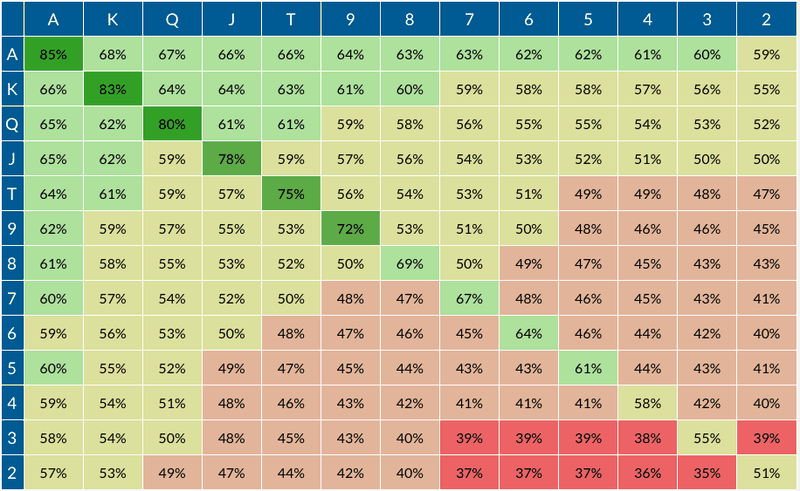
\includegraphics[scale=0.5]{images/preflop-chances.png}
\caption{Preflop kezek esélyei}
\cite{preflop-chances}
\label{fig:preflop-chances}
\end{figure}

\subsection{A felhasználó esélyeinek számítása}
Az egyszerűbb része az esélyek számolásának a felhasználó esélyeinek a kiszámolása, ugyanis itt kevesebbet kell számolni. 

A back end megkapja a front end-től a felhasználó által kiválasztott lapokat. Itt is definiálva van a pakli minden lapja, viszont objektum helyett csak egy tömbbe, mivel csak a lapok nevére van szükségünk. A default függvényben egy ellenőrzést végzek, hogy milyen hosszú az objektum, amit megkap. Erre azért van szükség, mert különböző számításokat kell végezni ha a flop-nál, turn-nél vagy river-nél szeretnénk megtudni esélyeinket. Először minden esetben a getOnlyName és a getJustDeck függvényeket használom. Az előbbivel az objektumot egy tömbre szűkítem, hogy csak a kártyák neveivel dolgozhassak tovább. Az utóbbival az összes lapot tartalmazó tömbből kitörlöm azokat, amelyeket a felhasználó már kiválasztott, így megkapom a pakliban maradt lapokat.

River esetében a tömb hosszúsága 7. Itt van a legegyszerűbb dolgom, mivel minden lap ismert, csak vissza kell térni a felhasználó kezének értékével. Először legenerálom a 7 lapból az összes 5 lap kombinációját, ezt a createCombinations függvénnyel teszem. Ez megkap egy 7 elemű tömböt és visszatér 21, 5 elemű tömbbel.A generációhoz a javascript generatorics nevű kombinatorikai könyvtárát használom.

\begin{python}
function createCombinations(sevenCards) {
  let allCombinations = [];
  for (let comb of G.combination(sevenCards, 5)) {
    allCombinations.push(comb.slice());
  }
  return allCombinations;
}
\end{python}

Ha megvan a 21, 5 elemű tömbünk, akkor már csak meg kell keresni mindegyiknek az értékét az adathalmazban, majd kiválasztani a legkissebbet és azzal visszatérni. Ezt a createStorngest függvény valósítja meg, amely megkapja az előbb említett 5 lapos kombinciókat és visszatér a legerősebb 5 lap értékével.

\begin{python}
function createStrongest(combinations){
  let rawdata = fs.readFileSync("data.json");
  let strenghtOrder = JSON.parse(rawdata);
  let result =  [];
  for (let combination of combinations) {
    let nameString = "";
    let colors = { C: 0, S: 0, H: 0, D: 0 };
    for (let card of combination) {
      nameString += card[0];
      colors[card[1]] += 1;
    }
    let ordered = sortCardOrder(nameString, colors);
    result.push(strenghtOrder.cardStrenght[ordered]);
  }
  return Math.min(...result);
}
\end{python}

A strengthOrder változóban eltárolom az adathalmazt. Egy foreach ciklussal végigmegyek mind a 21 kombináción. A cikluson belül ellenőrzöm, hogy a lapok között hány egyforma színű lap van, hiszen ha mind az 5 egyforma színű, akkor az olyan értékek közt is keresni kell, ahol számít a szín, tehát fulsh, esetleg színsorok. Itt a sortCardOrder függvény is szerepet játszik, itt rendezem abc sorrendbe a lapokat, illetve szúrok közé egy F betűt is, amennyiben figyelembe kell vennünk, hogy azonos színűek a lapok. A megkapott 21 lap értékével feltöltök egy tömböt, ezek után a függvény visszatér ennek a minimumával, ami a felhasználó lapjának az értéke lesz, ezt adom át a fornt end-nek.

Turn-nél a kapott tömb hosszúsága 6, azaz még egy lapra várunk, amely nem ismert. Ebben az esetben ugyanazt kell tenni, mint a river esetében, egy kiegészítéssel. Mivel egy lapra még várunk, így végig kell menni egy ciklussal az összes pakliban maradt kártyán, melyekkel kiegészítem a kapott tömbböt, és elvégzem ugyanazokat a számításokat, amiket a rivern-nél is. Mivel 46 lap maradt a pakliban, így 46 értékkel tér vissza a függvény, ezeket adom át a front end-nek.

Mikor három közös lap van az asztalon, azaz a flop, akkor egy 5 hosszúságú tömböt kap a back end, tehát még két lapra várunk.  Hasonló a teendő, mint az előző esetben, csak kicsit másképp. Mivel most két lapra várunk, így két egymásba ágyazott ciklusra van szükség, majd mindkettőnek az aktuális elemét hozzá kell fűzni a kapott tömbhöz, ezután meghívni ezekre a már ismert függvényeket, így megkapjuk az összes lehetséges lapra az esélyünket. A belső for ciklusnak mindig eggyel a külső for ciklus léptető változója előtt kell járnia, mivel így elkerülhetem, hogy egy adott kombináció kétféleképpen is előforduljon. Számunkra irreleváns, hogy a negyedik utcán érkezik egy treff király, az ötödiken pedig egy kör ász, vagy fordítva, a végeredmény ugyanaz.

Mikor csak a saját lapjainkat ismerjük, csupán annyit tesz az alkalmazás, hogy megkeresi a megadott két lapos kombinációt a PreflopData.json adathalmazban, és visszatér az értékével. Ez lesz a százalékos esélye a felhasználónak megnyerni a partit flop előtt. Ehhez a calcPreflopChance függvényt használja. Ebben szintén eltárolom egy változóba az adatokat, majd elvégzem a keresést benne. Ezen kívül annyi feladata van még, hogy ellenőrizze a két lap azonos színű-e. Ezt úgy teszi, hogy a lapok nevének a második karakterét, amely jelöli a színét, összehasonlítja. Amennyiben ezek egyenlőek, hozzáfűz egy F betűt, majd elvégzi a keresést az összefűzött string-el, valamint annak fordítottjával is. Erre azért van szükség, mert csak egy sorrendben szerepelnek a lapok a json dokumentumban, például az azonos színű ász-király AKf jelölésű, viszont ha mi először királyt kapunk, utána ászt, akkor a KAf jelölésre nem fog találni semmit.

\begin{python}
function calcPreflopChance(cards){
  let rawdata = fs.readFileSync("PreflopData.json");
  let chances = JSON.parse(rawdata);
  let cardCheck;
  let reversed;

  if(cards[0][1] == cards[1][1]){
    cardCheck = cards[0][0] + cards[1][0] + 'f';
    reversed = cards[1][0] + cards[0][0] + 'f'
  } else {
    cardCheck = cards[0][0] + cards[1][0]
    reversed = cards[1][0] + cards[0][0] 
  }

  if(chances['preflopStrenght'][cardCheck]){
    return chances['preflopStrenght'][cardCheck]
  } else {
    return chances['preflopStrenght'][reversed]
  }
}
\end{python}

\subsection{Ellenfél esélyeinek számítása}
Az ellenfél esélyeinek számítása egy kicsit bonyolultabb folyamat, mivel itt minden műveletnél 990-szer többet kell számolni, mint a saját esélyeinknél, hiszen az ellenfél kezében lévő két lapot nem ismerem.

Ez a rész sokban megegyezik az előző alszakaszban kifejtett részekkel. Itt is definiááltam a paklit, megkapjuk a front end-től a kiválasztott lapokat, valamint szintén a getOnlyName és getJustDeck függvényekkel kezdünk. Mivel többek között ezeket a függvényeket ez a file és az előzőekben tárgyalt is használja, így egy külön helperFunctions.js file-ban tárolom el, hogy ne kelljen mindkét file-ban kétszer megírni.

Ebben az esetben is az elágazás ágain szeretnék végigmenni, az elsőt részletesen bemutatni, majd a többit hozzá magyarázni. Első eset, mikor 7 hosszú a kapott tömb, tehát minden lapot ismerünk. Itt szükségem van az ellenfél 990 lehetséges lapjának az értékére. Ezt a createEnemysPossibleHands nevű függvény végzni.

\begin{python}
function createEnemysPossibleHands(allCards, sevenCardsName) {
  let eCombination = [];
  let everyCards = [...allCards];
  let allCombinations = [];
  for (let comb of G.combination(everyCards, 2)) {
    allCombinations.push(comb.slice());
  }
  for (let comb of allCombinations) {
    eCombination.push(comb.concat(sevenCardsName.slice(2, 7)));
  }
  return eCombination;
}
\end{python}

Ez a függvény megkapja az összes kártyát, ami még a pakliban maradt, valamint a kiválasztott hét lapot. A maradék lapokon végigmegy egy ciklussal és kiválasztja belőle az összes 2-es lap kombinációját, szintén a generatorics javascript könyvtár segítségével. Ezután ehhez a 2 laphoz hozzáfűzi a kapott tömb utolsó 5 elemét, hiszen ezek a közös lapok, amikkel keze alakulhat ki ellenfelünknek. Ezekkel az értékekkel visszatér.

A default függvényben egy foreach ciklussal végigmegyünk ezeken a 7 lapos kombinációkon. A cikluson belül hasonló módon, mint a felhasználó esélyeinek számításánál, legenerálom a 7-es kombinációkból az 5-ös kombinációkat, majd a legkissebb értékűvel számolok tovább. Így 990 értéket fogok kapni, az összes lehetséges 2 lapra, ami az ellenfélnél lehet. Ezután front end-en már csak annyi a dolgom, hogy összeshasonlítsam a felhasználó lapjáinak értékét ezzel a 990-el, és megkapom, hogy hány százalék esélye van nyerni a felhasználónak.

Ha még egy lapra várunk az asztalon, akkor az előbb említett lépéseket közrefogom egy for ciklussal, mely végigmegy a pakli lapjain és az adott lappal kiegészíti a tömböt. Hasonló módon, mint a felhasználó esélyeinek számításánál, annyi különbséggel, hogy itt ügyelni kell a lap tömbből való kitörlésére is, hiszem a számításokat végző függvények megkapják a 7 lap mellett a pakliban maradt lapokat is. A törlést a removeItemOnce függvény végzi, mely szintén a helperFunctions-ben található, hiszen mindkét file-ban felhasználom.

\begin{python}
export function removeItemOnce(arr, value) {
    let arrCopy = arr;
    var index = arrCopy.indexOf(value);
    if (index > -1) {
      arrCopy.splice(index, 1);
    }
    return arrCopy;
}
\end{python}

Flop esetében csakúgy mint eddig, két egymásba ágyazott for ciklussal valósítom meg a maradék két lap érkezését. Szintén a belső ciklus eggyel előrébbről indul, mint a külső az ismétlődés elkerülése végett. Ilyenkor az 5 laphoz mindkét ciklusnál hozzáfűzzöm az adott kártyát, valamint kitörlöm a tömbből. Ezekre a tömbökre elvégzem ugyanazokat a lépéseket, mint eddig és megkapom az ellenfél összes lehetséges lapjára az értéket. Ugyanígy összehasonlítom a felhasználó várható értékeivel laponként, majd ábrázolom a diagramon.

\section{Kapcsolat a back end és a front end között}
A back end és a front end közötti kapcsolatot két fügvénnyel valósítom meg, amelyekben egy-egy POST request szerepel. Mindkét esetben a body-ban átadom a sevenCards objektumot, amely tartalmazza a felhasználó által kiválasztott lapokat. Az egyik esetben a fetch-ben a mystrongest, a másikban az enemystrongest szerepel. A back end mindig az 5000-es porton kommunikál a fornt end-el.

\begin{python}
backendOfMyCards(e) {
      e.preventDefault();
      fetch("http://localhost:5000/mystrongest", {
        method: "POST",
        headers: { "Content-Type": "application/json" },
        body: JSON.stringify({ sevenCards: this.sevenCards }),
      })
        .then((res) => {
          return res.json();
        })
        .then((json) => {
          (this.myCards = json);
        });
    },
\end{python}

A függvény visszatér a back end-től kapott adatokkal, valamint a myCards tömmbe kerülnek a felhasználó esélyei. Az ellenfél esélyeinél természetesen az ő esélyeivel tér vissza a függvény, és az enemyCards tömböt tölti fel.

Szerver oldalról a root.js file-ban található az a rész, amely a kapcsolatot végzi a kliens oldallal. Ide importáltam a findStrongest.js és findEnemyStrongest.js file-okat. Itt két POST response található. A különbség a kettő között, hogy míg az egyik a fent említett file-ok közül ez előbbit, a másik az utóbbit valósítja meg és küldi vissza. Egy változóba eltárolom a front end kérés body részét, erre meghívom az adott függvényt és ezzel vissza is küldöm a front end-nek.

\begin{python}
router.post('/mystrongest', (req, res, next) => {
    let cards = req.body;
    res.setHeader("Content-Type", "application/json")
    res.json(findStrongest(cards)).send();
});
\end{python}